\subsection{Localisation of Exogenously Expressed IFITs During RSV Infection} \label{subsec:Localisation of Exogenously Expressed IFITs During RSV Infection}

\lipsum[1-30]



\subsubsection{Overexpressed Human IFIT1 During hRSV and bRSV Infection}
Overexpressed hIFIT1-FLAG colocalises with both human and bovine RSV IBs. This data is supported by evidence from z stacks.

\begin{figure}
    \begin{subfigure}{0.495\textwidth}
        \caption{}
        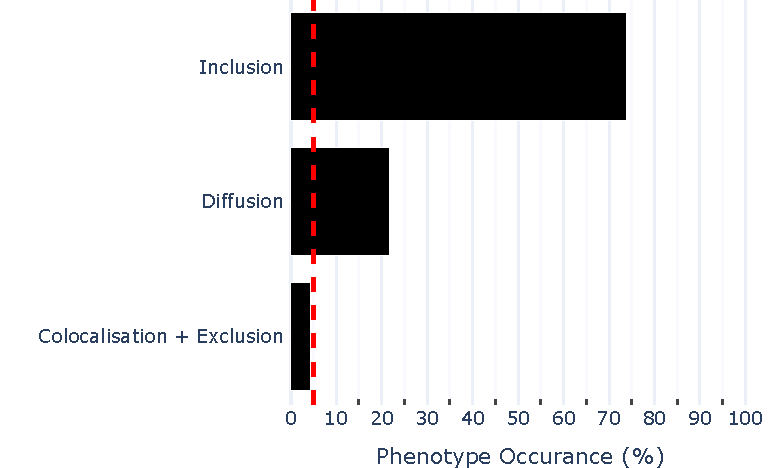
\includegraphics[width=1\linewidth]{08. Chapter 3/Figs/04. Overexpression/01. IFIT1/01. bar_i1_hrsv.pdf} 
    \end{subfigure}
    \begin{subfigure}{0.495\textwidth}
        \caption{}
        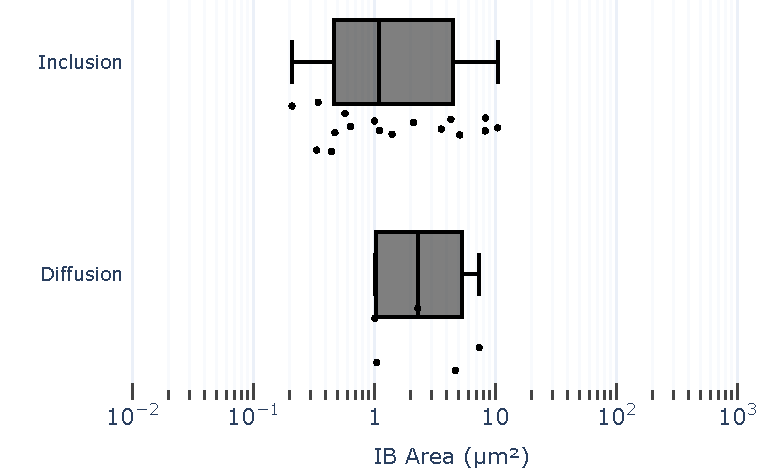
\includegraphics[width=1\linewidth]{08. Chapter 3/Figs/04. Overexpression/01. IFIT1/02. box_i1_hrsv.pdf}
    \end{subfigure}
    \caption[Observed Phenotypes of Exogenous hIFIT1 in the Context of hRSV Inclusion Bodies in VERO Cell Line.]{\textbf{Observed Phenotypes of Exogenous hIFIT1 in the Context of hRSV Inclusion Bodies in VERO Cell Line.} Vero cells were infected with human RSV at MOI 1. 24 HPI, the cells were transfected with hIFIT1-FLAG containing plasmids using TransIT-X2 and were fixed after further 24 hours. Cells were labeled with anti-RSV N and anti-FLAG antibodies and imaged on confocal microscope. Panel (a) shows percentual proportions of observed phenotypes between hRSV inclusion bodies and exogenous hIFIT1 (23 observations), with the red dotted line denoting the 5\% threshold, marking phenotypes considered relevant above this limit. Panel (b) shows the IB area in \(\mu m^2\) per observed relevant phenotype.}
    \label{fig:Observed Phenotypes of Exogenous hIFIT1 in the Context of hRSV Inclusion Bodies in VERO Cell Line}
\end{figure}

\begin{figure}
    \centering
    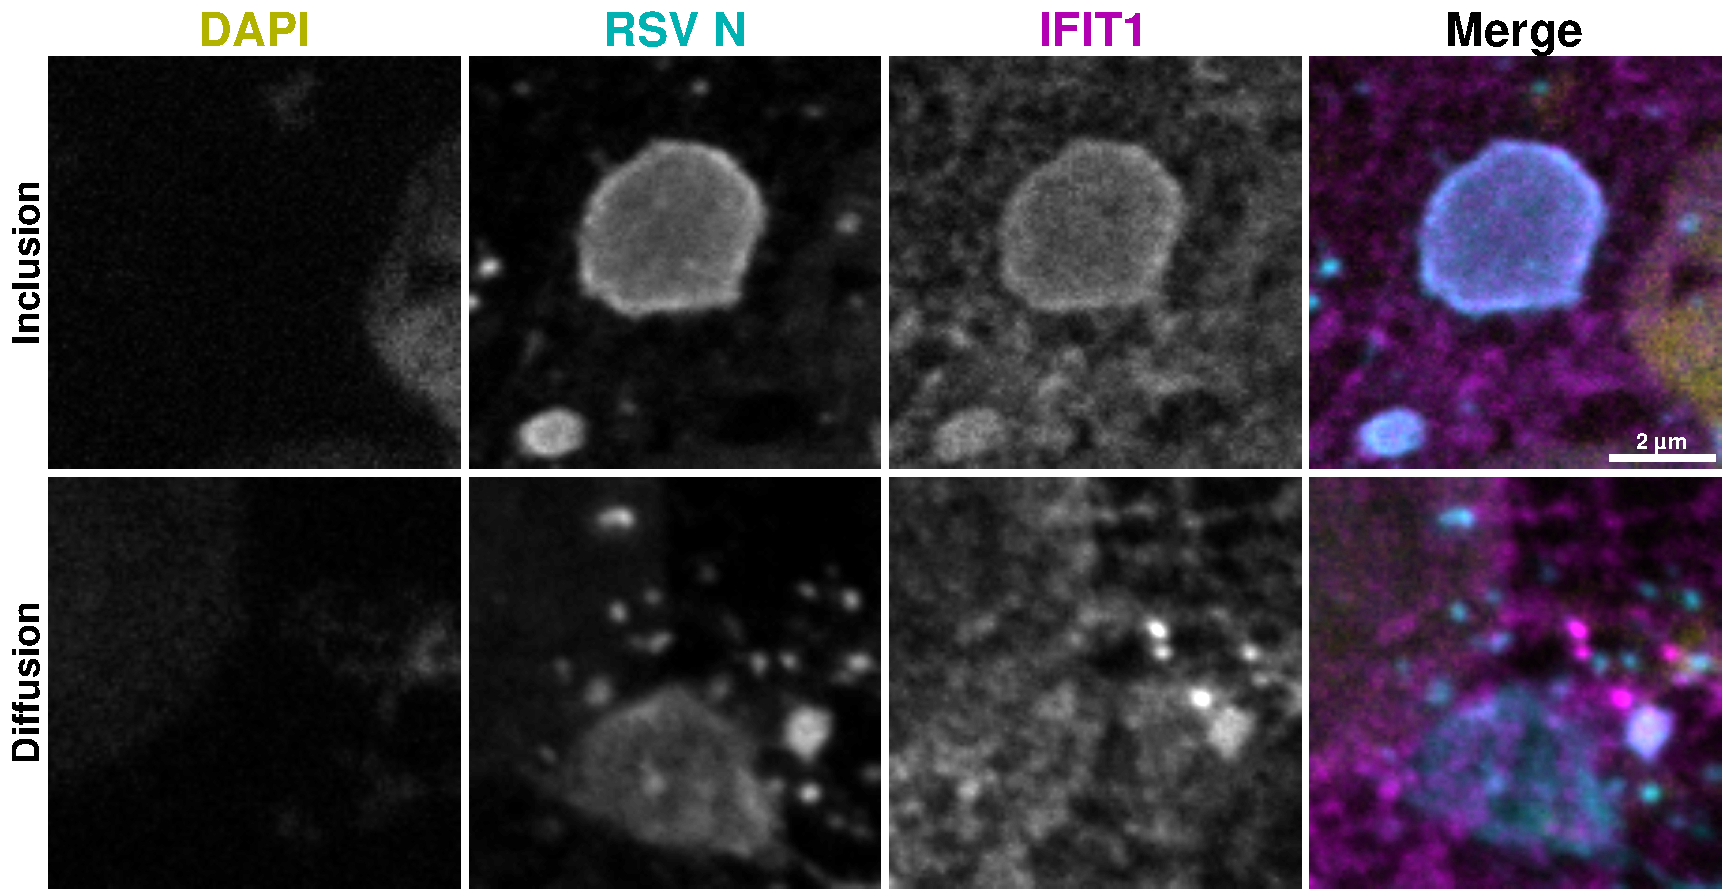
\includegraphics[width=1\linewidth]{08. Chapter 3/Figs/04. Overexpression/01. IFIT1/03. i1-hrsv.pdf}
    \caption[Representative Images of Observed Phenotypes of Exogenous hIFIT1 in the Context of hRSV Inclusion Bodies in VERO Cell Line.]{\textbf{Representative Images of Observed Phenotypes of Exogenous hIFIT1 in the Context of hRSV Inclusion Bodies in VERO Cell Line.} Vero cells were infected with human RSV at MOI 1. 24 HPI, the cells were transfected with hIFIT1-FLAG containing plasmids using TransIT-X2 and were fixed after further 24 hours. Cellular nuclei were stained with DAPI (yellow), and cells were double-labeled with anti-RSV N (cyan) and anti-FLAG (magenta) antibodies. This figure showcases representative examples of relevant phenotypes in the interaction between exogenous hIFIT1 and hRSV inclusion bodies. These phenotypes are presented in descending order based on their percentage proportions. The scale bar indicates 2 \(\mu m\).}
    \label{fig:Representative Images of Observed Phenotypes of Exogenous hIFIT1 in the Context of hRSV Inclusion Bodies in VERO Cell Line}
\end{figure}

74 21

1.1 2.2

\begin{figure}
    \begin{subfigure}{0.495\textwidth}
        \caption{}
        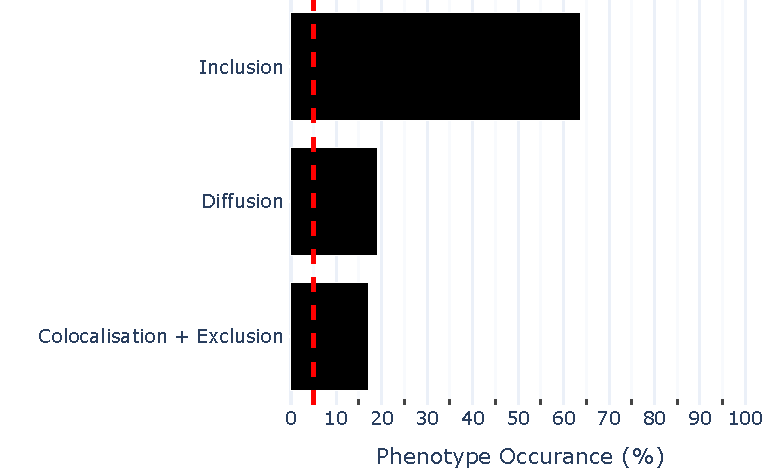
\includegraphics[width=1\linewidth]{08. Chapter 3/Figs/04. Overexpression/01. IFIT1/04. bar_i1_brsv.pdf} 
    \end{subfigure}
    \begin{subfigure}{0.495\textwidth}
        \caption{}
        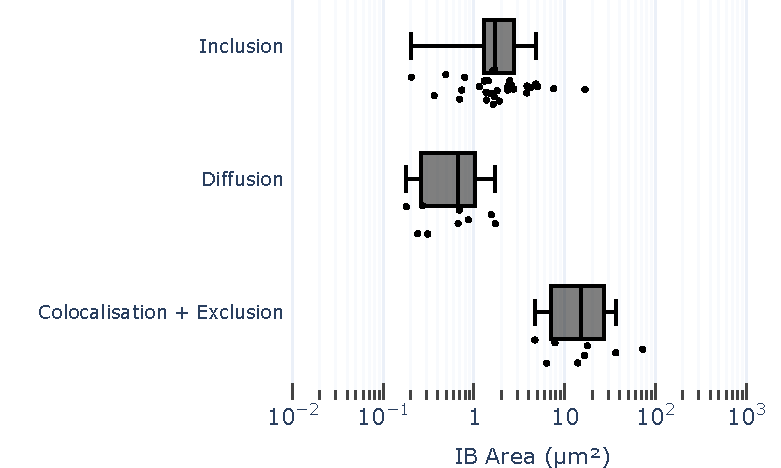
\includegraphics[width=1\linewidth]{08. Chapter 3/Figs/04. Overexpression/01. IFIT1/05. box_i1_brsv.pdf}
    \end{subfigure}
    \caption[Observed Phenotypes of Exogenous hIFIT1 in the Context of bRSV Inclusion Bodies in VERO Cell Line.]{\textbf{Observed Phenotypes of Exogenous hIFIT1 in the Context of bRSV Inclusion Bodies in VERO Cell Line.} Vero cells were infected with bovine RSV at MOI 1. 24 HPI, the cells were transfected with hIFIT1-FLAG containing plasmids using TransIT-X2 and were fixed after further 24 hours. Cells were labeled with anti-RSV N and anti-FLAG antibodies and imaged on confocal microscope. Panel (a) shows percentual proportions of observed phenotypes between bRSV inclusion bodies and exogenous hIFIT1 (47 observations), with the red dotted line denoting the 5\% threshold, marking phenotypes considered relevant above this limit. Panel (b) shows the IB area in \(\mu m^2\) per observed relevant phenotype.}
    \label{fig:Observed Phenotypes of Exogenous hIFIT1 in the Context of bRSV Inclusion Bodies in VERO Cell Line}
\end{figure}

\begin{figure}
    \centering
    \includegraphics[width=1\linewidth]{08. Chapter 3/Figs/04. Overexpression/01. IFIT1/06. i1-brsv.pdf}
    \caption[Representative Images of Observed Phenotypes of Exogenous hIFIT1 in the Context of bRSV Inclusion Bodies in VERO Cell Line.]{\textbf{Representative Images of Observed Phenotypes of Exogenous hIFIT1 in the Context of bRSV Inclusion Bodies in VERO Cell Line.} Vero cells were infected with bovine RSV at MOI 1. 24 HPI, the cells were transfected with hIFIT1-FLAG containing plasmids using TransIT-X2 and were fixed after further 24 hours. Cellular nuclei were stained with DAPI (yellow), and cells were double-labeled with anti-RSV N (cyan) and anti-FLAG (magenta) antibodies. This figure showcases representative examples of relevant phenotypes in the interaction between exogenous hIFIT1 and bRSV inclusion bodies. These phenotypes are presented in descending order based on their percentage proportions. The scale bar indicates 2 \(\mu m\).}
    \label{fig:Representative Images of Observed Phenotypes of Exogenous hIFIT1 in the Context of bRSV Inclusion Bodies in VERO Cell Line}
\end{figure}

64 19 16

1.8, 0.8, 14

\subsubsection{Overexpressed Human and Bovine IFIT2 During hRSV and bRSV Infection}

\begin{figure}
    \begin{subfigure}{0.495\textwidth}
        \caption{}
        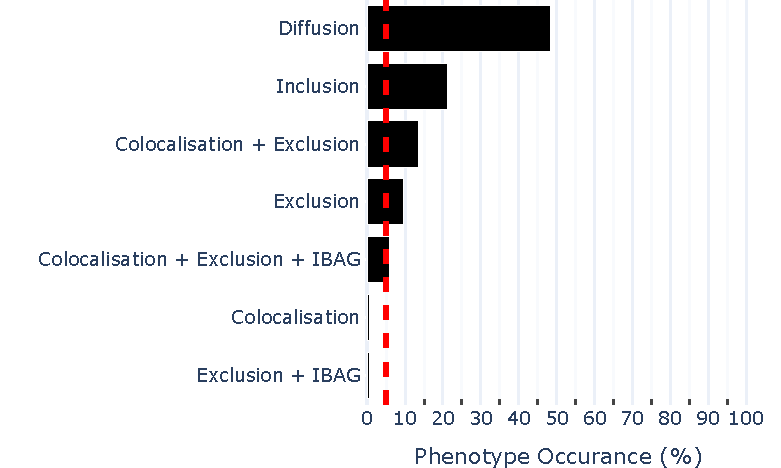
\includegraphics[width=1\linewidth]{08. Chapter 3/Figs/04. Overexpression/02. IFIT2/01. bar_hi2f_hrsv.pdf} 
    \end{subfigure}
    \begin{subfigure}{0.495\textwidth}
        \caption{}
        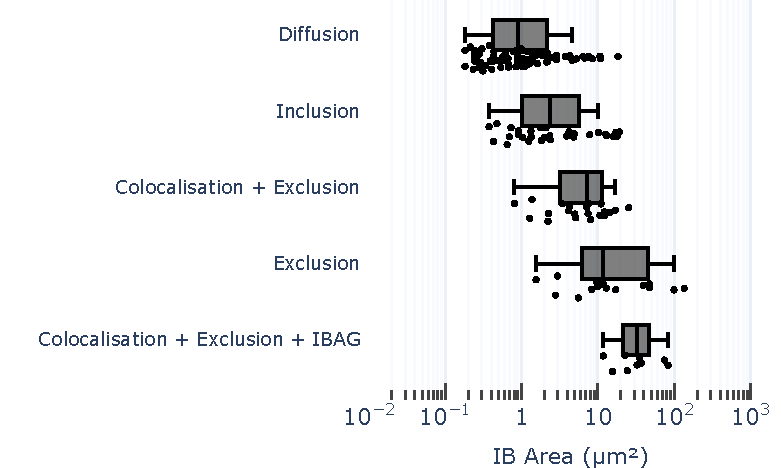
\includegraphics[width=1\linewidth]{08. Chapter 3/Figs/04. Overexpression/02. IFIT2/02. box_hi2f_hrsv.pdf}
    \end{subfigure}
    \caption[Observed Phenotypes of Exogenous hIFIT2 in the Context of hRSV Inclusion Bodies in VERO Cell Line.]{\textbf{Observed Phenotypes of Exogenous hIFIT2 in the Context of hRSV Inclusion Bodies in VERO Cell Line.} Vero cells were infected with human RSV at MOI 1. 24 HPI, the cells were transfected with hIFIT2-FLAG containing plasmids using TransIT-X2 and were fixed after further 24 hours. Cells were labeled with anti-RSV N and anti-FLAG antibodies and imaged on confocal microscope. Panel (a) shows percentual proportions of observed phenotypes between hRSV inclusion bodies and exogenous hIFIT2 (155 observations), with the red dotted line denoting the 5\% threshold, marking phenotypes considered relevant above this limit. Panel (b) shows the IB area in \(\mu m^2\) per observed relevant phenotype.}
    \label{fig:Observed Phenotypes of Exogenous hIFIT2 in the Context of hRSV Inclusion Bodies in VERO Cell Line}
\end{figure}

\begin{figure}
    \centering
    \includegraphics[width=1\linewidth]{08. Chapter 3/Figs/04. Overexpression/02. IFIT2/03. hi2f-hrsv.pdf}
    \caption[Representative Images of Observed Phenotypes of Exogenous hIFIT2 in the Context of hRSV Inclusion Bodies in VERO Cell Line.]{\textbf{Representative Images of Observed Phenotypes of Exogenous hIFIT2 in the Context of hRSV Inclusion Bodies in VERO Cell Line.} Vero cells were infected with human RSV at MOI 1. 24 HPI, the cells were transfected with hIFIT2-FLAG containing plasmids using TransIT-X2 and were fixed after further 24 hours. Cellular nuclei were stained with DAPI (yellow), and cells were double-labeled with anti-RSV N (cyan) and anti-FLAG (magenta) antibodies. This figure showcases representative examples of relevant phenotypes in the interaction between exogenous hIFIT2 and hRSV inclusion bodies. These phenotypes are presented in descending order based on their percentage proportions. The scale bar indicates 2 \(\mu m\).}
    \label{fig:Representative Images of Observed Phenotypes of Exogenous hIFIT2 in the Context of hRSV Inclusion Bodies in VERO Cell Line}
\end{figure}

48 21 14 9 5
0.9 2.1 7 11 32

In the follow up experiment, exogenous bovine IFIT2 in the context of human RSV infection shows the same two phenotypes. It is either excluded from the IBs (middle panel) or colocalises with the ring structure of the IBs (top and bottom panel; highlighted with arrows).

\begin{figure}
    \begin{subfigure}{0.495\textwidth}
        \caption{}
        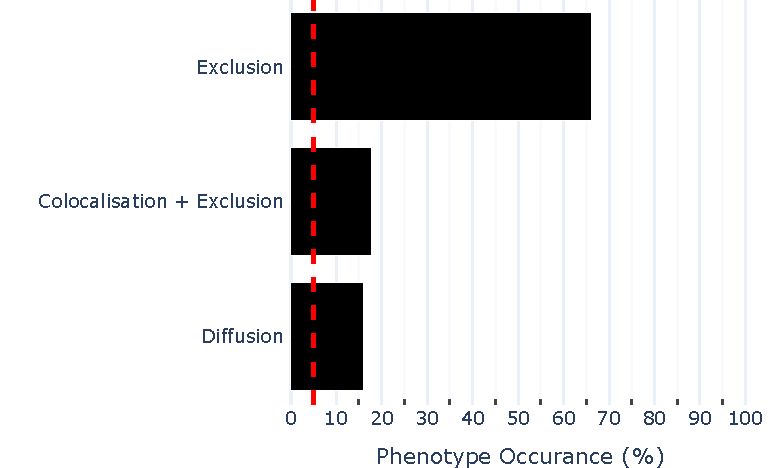
\includegraphics[width=1\linewidth]{08. Chapter 3/Figs/04. Overexpression/02. IFIT2/04. bar_bi2f_hrsv.pdf} 
    \end{subfigure}
    \begin{subfigure}{0.495\textwidth}
        \caption{}
        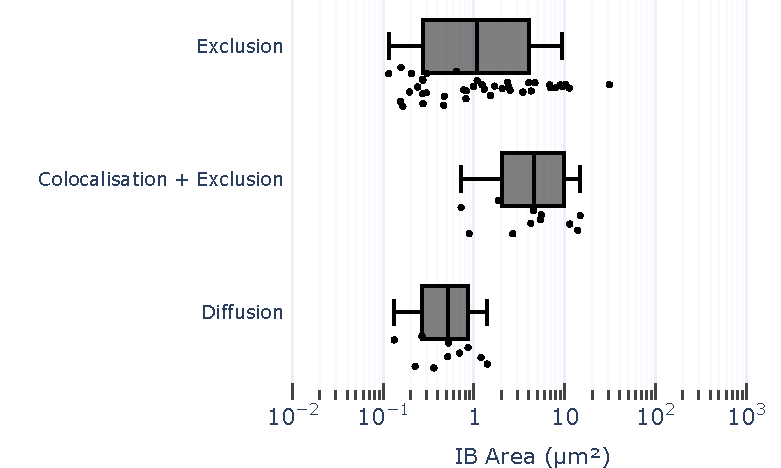
\includegraphics[width=1\linewidth]{08. Chapter 3/Figs/04. Overexpression/02. IFIT2/05. box_bi2f_hrsv.pdf}
    \end{subfigure}
    \caption[Observed Phenotypes of Exogenous bIFIT2 in the Context of hRSV Inclusion Bodies in VERO Cell Line.]{\textbf{Observed Phenotypes of Exogenous bIFIT2 in the Context of hRSV Inclusion Bodies in VERO Cell Line.} Vero cells were infected with human RSV at MOI 1. 24 HPI, the cells were transfected with bIFIT2-FLAG containing plasmids using TransIT-X2 and were fixed after further 24 hours. Cells were labeled with anti-RSV N and anti-FLAG antibodies and imaged on confocal microscope. Panel (a) shows percentual proportions of observed phenotypes between hRSV inclusion bodies and exogenous bIFIT2 (62 observations), with the red dotted line denoting the 5\% threshold, marking phenotypes considered relevant above this limit. Panel (b) shows the IB area in \(\mu m^2\) per observed relevant phenotype.}
    \label{fig:Observed Phenotypes of Exogenous bIFIT2 in the Context of hRSV Inclusion Bodies in VERO Cell Line}
\end{figure}

\begin{figure}
    \centering
    \includegraphics[width=1\linewidth]{08. Chapter 3/Figs/04. Overexpression/02. IFIT2/06. bi2f-hrsv.pdf}
    \caption[Representative Images of Observed Phenotypes of Exogenous bIFIT2 in the Context of hRSV Inclusion Bodies in VERO Cell Line.]{\textbf{Representative Images of Observed Phenotypes of Exogenous bIFIT2 in the Context of hRSV Inclusion Bodies in VERO Cell Line.} Vero cells were infected with human RSV at MOI 1. 24 HPI, the cells were transfected with bIFIT2-FLAG containing plasmids using TransIT-X2 and were fixed after further 24 hours. Cellular nuclei were stained with DAPI (yellow), and cells were double-labeled with anti-RSV N (cyan) and anti-FLAG (magenta) antibodies. This figure showcases representative examples of relevant phenotypes in the interaction between exogenous bIFIT2 and hRSV inclusion bodies. These phenotypes are presented in descending order based on their percentage proportions. The scale bar indicates 2 \(\mu m\).}
    \label{fig:Representative Images of Observed Phenotypes of Exogenous bIFIT2 in the Context of hRSV Inclusion Bodies in VERO Cell Line}
\end{figure}

66 17 16
1 5 0.5

Exogenous bovine IFIT2 during bovine RSV infection seems to be excluded from the inclusion bodies, although the data is not great and the IFIT2 is aggregated in both cells shown.

\begin{figure}
    \begin{subfigure}{0.495\textwidth}
        \caption{}
        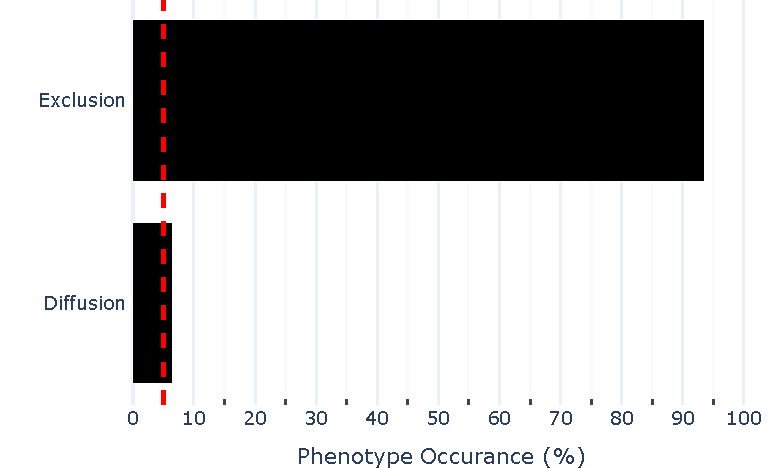
\includegraphics[width=1\linewidth]{08. Chapter 3/Figs/04. Overexpression/02. IFIT2/07. bar_bi2f_brsv.pdf} 
    \end{subfigure}
    \begin{subfigure}{0.495\textwidth}
        \caption{}
        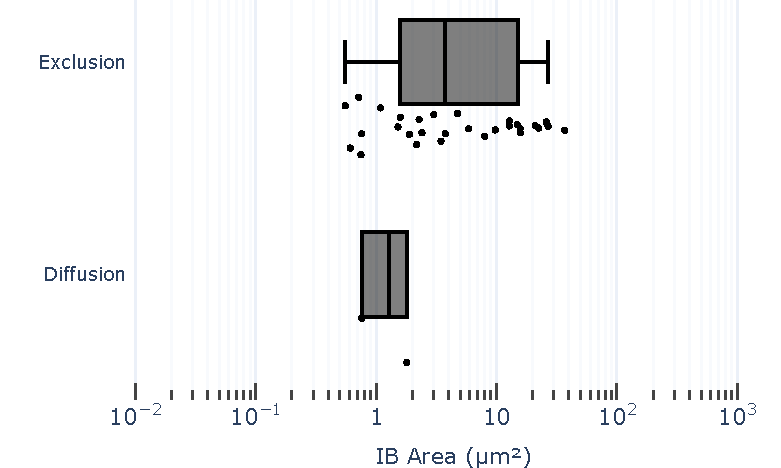
\includegraphics[width=1\linewidth]{08. Chapter 3/Figs/04. Overexpression/02. IFIT2/08. box_bi2f_brsv.pdf}
    \end{subfigure}
    \caption[Observed Phenotypes of Exogenous bIFIT2 in the Context of bRSV Inclusion Bodies in VERO Cell Line.]{\textbf{Observed Phenotypes of Exogenous bIFIT2 in the Context of bRSV Inclusion Bodies in VERO Cell Line.} Vero cells were infected with human RSV at MOI 1. 24 HPI, the cells were transfected with bIFIT2-FLAG containing plasmids using TransIT-X2 and were fixed after further 24 hours. Cells were labeled with anti-RSV N and anti-FLAG antibodies and imaged on confocal microscope. Panel (a) shows percentual proportions of observed phenotypes between bRSV inclusion bodies and exogenous bIFIT2 (31 observations), with the red dotted line denoting the 5\% threshold, marking phenotypes considered relevant above this limit. Panel (b) shows the IB area in \(\mu m^2\) per observed relevant phenotype.}
    \label{fig:Observed Phenotypes of Exogenous bIFIT2 in the Context of bRSV Inclusion Bodies in VERO Cell Line}
\end{figure}

\begin{figure}
    \centering
    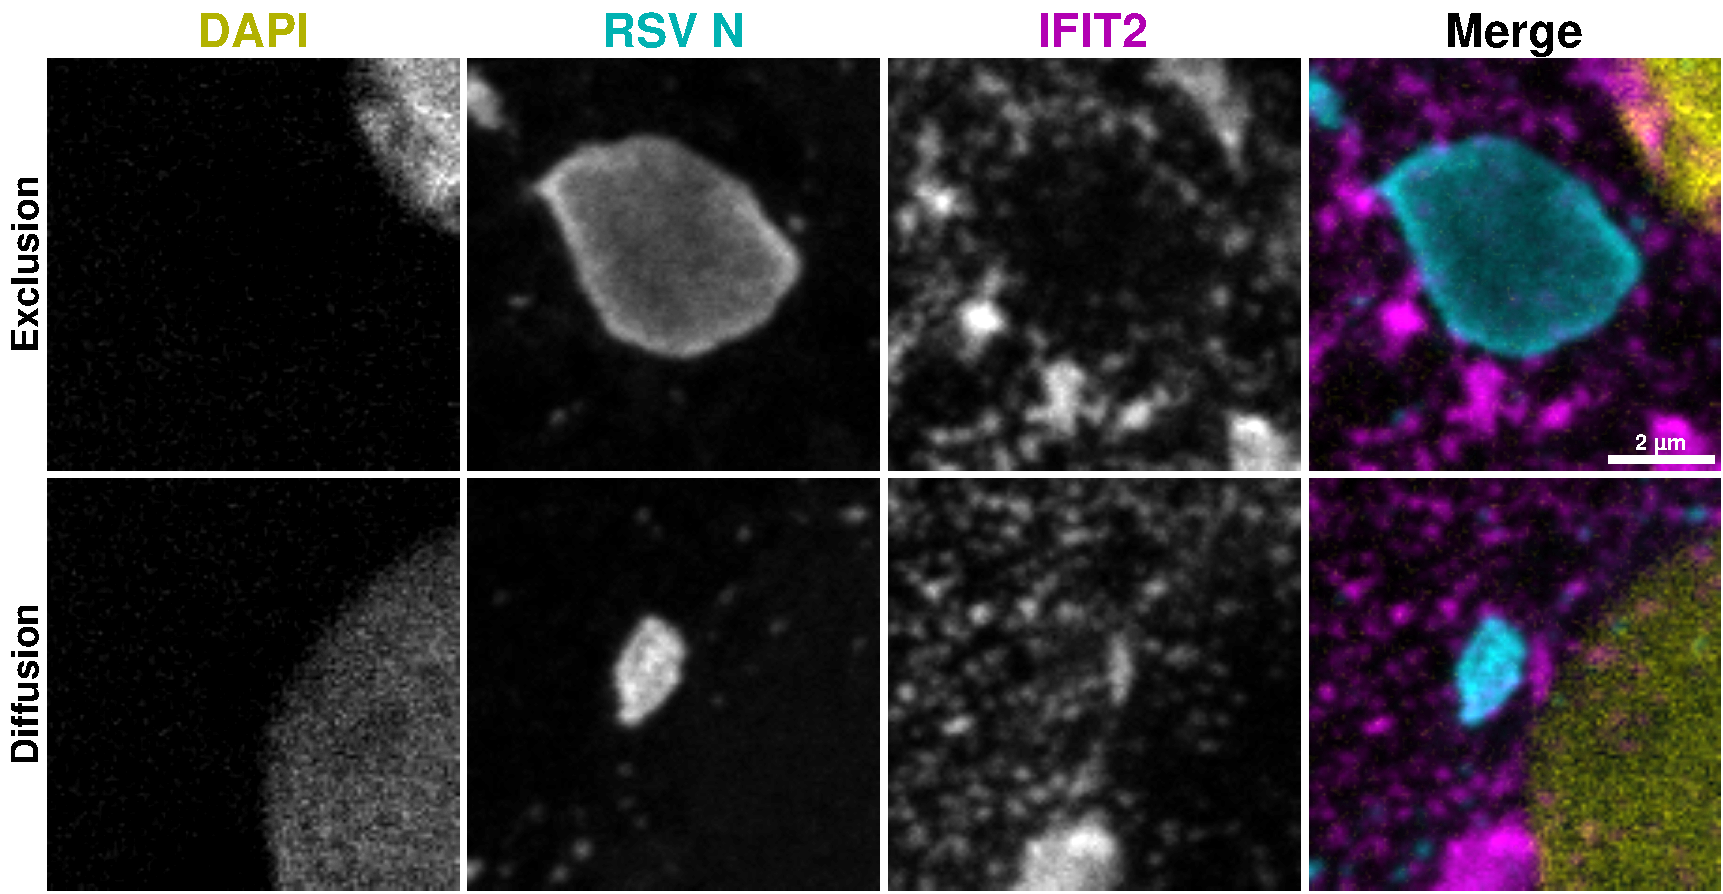
\includegraphics[width=1\linewidth]{08. Chapter 3/Figs/04. Overexpression/02. IFIT2/09. bi2f-brsv.pdf}
    \caption[Representative Images of Observed Phenotypes of Exogenous bIFIT2 in the Context of bRSV Inclusion Bodies in VERO Cell Line.]{\textbf{Representative Images of Observed Phenotypes of Exogenous bIFIT2 in the Context of bRSV Inclusion Bodies in VERO Cell Line.} Vero cells were infected with human RSV at MOI 1. 24 HPI, the cells were transfected with bIFIT2-FLAG containing plasmids using TransIT-X2 and were fixed after further 24 hours. Cellular nuclei were stained with DAPI (yellow), and cells were double-labeled with anti-RSV N (cyan) and anti-FLAG (magenta) antibodies. This figure showcases representative examples of relevant phenotypes in the interaction between exogenous bIFIT2 and bRSV inclusion bodies. These phenotypes are presented in descending order based on their percentage proportions. The scale bar indicates 2 \(\mu m\).}
    \label{fig:Representative Images of Observed Phenotypes of Exogenous bIFIT2 in the Context of bRSV Inclusion Bodies in VERO Cell Line}
\end{figure}

94 6
3.9 1.3

\subsubsection{Overexpressed Bovine IFIT3 During hRSV and bRSV Infection}
Overexpressed bIFIT3-FLAG was observed to colocalise with hRSV inclusion bodies (top panel; highlighted with arrows), as well as being excluded from the hRSV IBs, without any signs of IFIT3 signal on the periphery of the IB structures (middle and bottom panel). This data is supported by z stack measurements.

\begin{figure}
    \begin{subfigure}{0.495\textwidth}
        \caption{}
        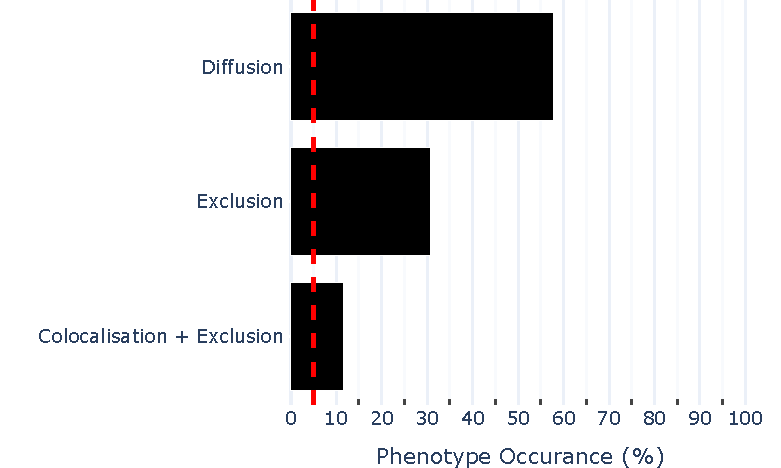
\includegraphics[width=1\linewidth]{08. Chapter 3/Figs/04. Overexpression/03. IFIT3/01. bar_i3_hrsv.pdf} 
    \end{subfigure}
    \begin{subfigure}{0.495\textwidth}
        \caption{}
        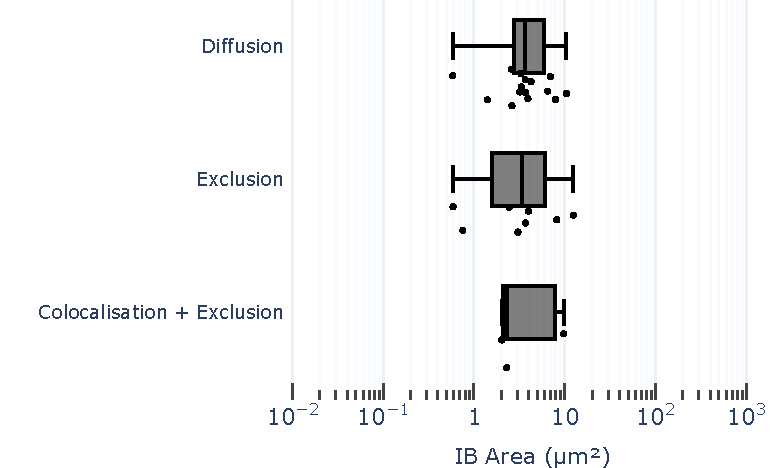
\includegraphics[width=1\linewidth]{08. Chapter 3/Figs/04. Overexpression/03. IFIT3/02. box_i3_hrsv.pdf}
    \end{subfigure}
    \caption[Observed Phenotypes of Exogenous bIFIT3 in the Context of hRSV Inclusion Bodies in VERO Cell Line.]{\textbf{Observed Phenotypes of Exogenous bIFIT3 in the Context of hRSV Inclusion Bodies in VERO Cell Line.} Vero cells were infected with human RSV at MOI 1. 24 HPI, the cells were transfected with bIFIT3-FLAG containing plasmids using TransIT-X2 and were fixed after further 24 hours. Cells were labeled with anti-RSV N and anti-FLAG antibodies and imaged on confocal microscope. Panel (a) shows percentual proportions of observed phenotypes between hRSV inclusion bodies and exogenous bIFIT3 (26 observations), with the red dotted line denoting the 5\% threshold, marking phenotypes considered relevant above this limit. Panel (b) shows the IB area in \(\mu m^2\) per observed relevant phenotype.}
    \label{fig:Observed Phenotypes of Exogenous bIFIT3 in the Context of hRSV Inclusion Bodies in VERO Cell Line}
\end{figure}

\begin{figure}
    \centering
    \includegraphics[width=1\linewidth]{08. Chapter 3/Figs/04. Overexpression/03. IFIT3/03. bi3-hrsv.pdf}
    \caption[Representative Images of Observed Phenotypes of Exogenous bIFIT3 in the Context of hRSV Inclusion Bodies in VERO Cell Line.]{\textbf{Representative Images of Observed Phenotypes of Exogenous bIFIT3 in the Context of hRSV Inclusion Bodies in VERO Cell Line.} Vero cells were infected with human RSV at MOI 1. 24 HPI, the cells were transfected with bIFIT3-FLAG containing plasmids using TransIT-X2 and were fixed after further 24 hours. Cellular nuclei were stained with DAPI (yellow), and cells were double-labeled with anti-RSV N (cyan) and anti-FLAG (magenta) antibodies. This figure showcases representative examples of relevant phenotypes in the interaction between exogenous bIFIT3 and hRSV inclusion bodies. These phenotypes are presented in descending order based on their percentage proportions. The scale bar indicates 2 \(\mu m\).}
    \label{fig:Representative Images of Observed Phenotypes of Exogenous bIFIT3 in the Context of hRSV Inclusion Bodies in VERO Cell Line}
\end{figure}

57 31 12

4, 3.3, 2.1

Very similar phenotype is observed for overexpressed bIFIT3-FLAG in bRSV infected cells. We see colocalization with IB (top panel) as well as exclusion from the structure without any signs of IFIT3 signal on the periphery of the IB structure (bottom panel). This data is as well supported by z stack measurements.

\begin{figure}
    \begin{subfigure}{0.495\textwidth}
        \caption{}
        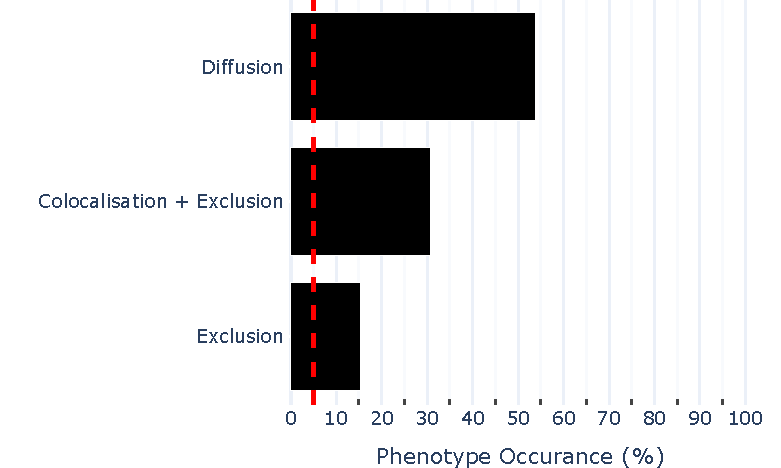
\includegraphics[width=1\linewidth]{08. Chapter 3/Figs/04. Overexpression/03. IFIT3/04. bar_i3_brsv.pdf} 
    \end{subfigure}
    \begin{subfigure}{0.495\textwidth}
        \caption{}
        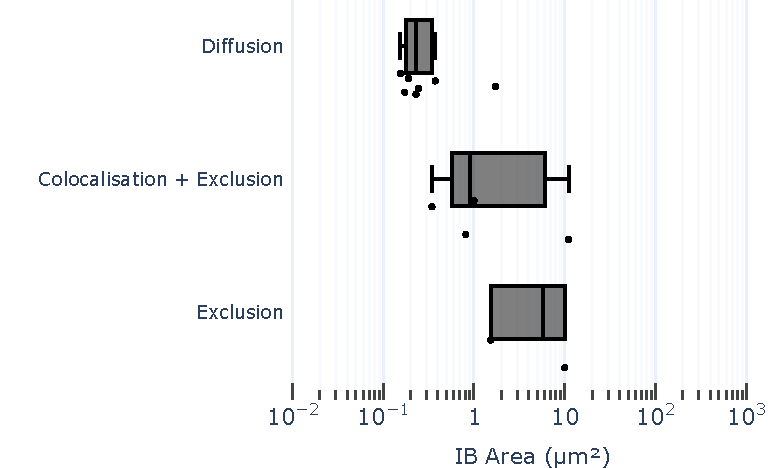
\includegraphics[width=1\linewidth]{08. Chapter 3/Figs/04. Overexpression/03. IFIT3/05. box_i3_brsv.pdf}
    \end{subfigure}
    \caption[Observed Phenotypes of Exogenous bIFIT3 in the Context of bRSV Inclusion Bodies in VERO Cell Line.]{\textbf{Observed Phenotypes of Exogenous bIFIT3 in the Context of bRSV Inclusion Bodies in VERO Cell Line.} Vero cells were infected with bovine RSV at MOI 1. 24 HPI, the cells were transfected with bIFIT3-FLAG containing plasmids using TransIT-X2 and were fixed after further 24 hours. Cells were labeled with anti-RSV N and anti-FLAG antibodies and imaged on confocal microscope. Panel (a) shows percentual proportions of observed phenotypes between bRSV inclusion bodies and exogenous bIFIT3 (13 observations), with the red dotted line denoting the 5\% threshold, marking phenotypes considered relevant above this limit. Panel (b) shows the IB area in \(\mu m^2\) per observed relevant phenotype.}
    \label{fig:Observed Phenotypes of Exogenous bIFIT3 in the Context of bRSV Inclusion Bodies in VERO Cell Line}
\end{figure}

\begin{figure}
    \centering
    \includegraphics[width=1\linewidth]{08. Chapter 3/Figs/04. Overexpression/03. IFIT3/06. bi3-brsv.pdf}
    \caption[Representative Images of Observed Phenotypes of Exogenous bIFIT3 in the Context of bRSV Inclusion Bodies in VERO Cell Line.]{\textbf{Representative Images of Observed Phenotypes of Exogenous bIFIT3 in the Context of bRSV Inclusion Bodies in VERO Cell Line.} Vero cells were infected with bovine RSV at MOI 1. 24 HPI, the cells were transfected with bIFIT3-FLAG containing plasmids using TransIT-X2 and were fixed after further 24 hours. Cellular nuclei were stained with DAPI (yellow), and cells were double-labeled with anti-RSV N (cyan) and anti-FLAG (magenta) antibodies. This figure showcases representative examples of relevant phenotypes in the interaction between exogenous bIFIT3 and bRSV inclusion bodies. These phenotypes are presented in descending order based on their percentage proportions. The scale bar indicates 2 \(\mu m\).}
    \label{fig:Representative Images of Observed Phenotypes of Exogenous bIFIT3 in the Context of bRSV Inclusion Bodies in VERO Cell Line}
\end{figure}

54 31 15

0.22 0.9 6



\subsubsection{Overexpressed Human IFIT5 During hRSV and bRSV Infection}
hIFIT5-FLAG is colocalising with hRSV inclusion bodies (basically resembling the P staining), while in bRSV infected cell there is a hint of IFIT5 signal concentration at the side of bRSV IB.

This data is by single cells per conditions as transfection did not work well. It is however supported by z stack measurements.

\begin{figure}
    \begin{subfigure}{0.495\textwidth}
        \caption{}
        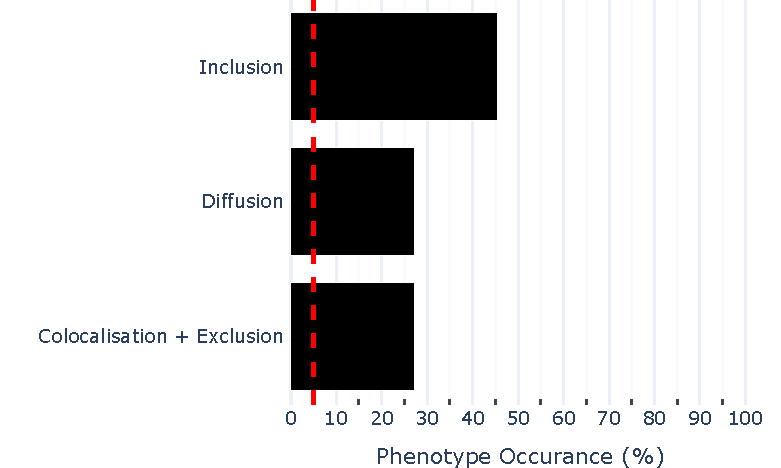
\includegraphics[width=1\linewidth]{08. Chapter 3/Figs/04. Overexpression/04. IFIT5/01. bar_i5_hrsv.pdf} 
    \end{subfigure}
    \begin{subfigure}{0.495\textwidth}
        \caption{}
        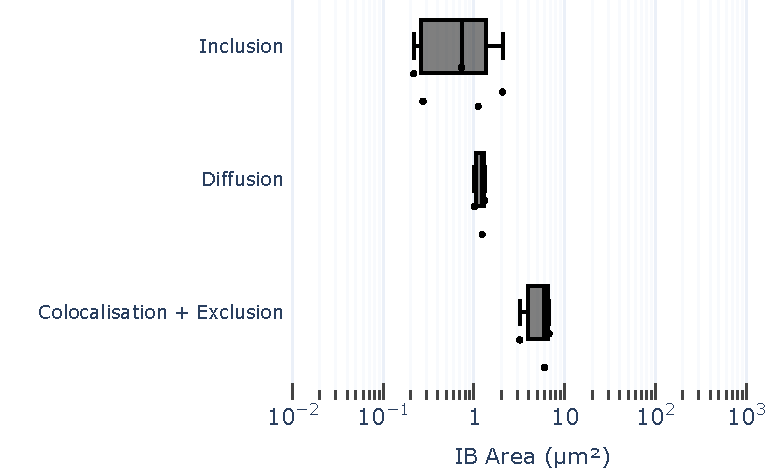
\includegraphics[width=1\linewidth]{08. Chapter 3/Figs/04. Overexpression/04. IFIT5/02. box_i5_hrsv.pdf}
    \end{subfigure}
    \caption[Observed Phenotypes of Exogenous hIFIT5 in the Context of hRSV Inclusion Bodies in VERO Cell Line.]{\textbf{Observed Phenotypes of Exogenous hIFIT5 in the Context of hRSV Inclusion Bodies in VERO Cell Line.} Vero cells were infected with human RSV at MOI 1. 24 HPI, the cells were transfected with hIFIT5-FLAG containing plasmids using TransIT-X2 and were fixed after further 24 hours. Cells were labeled with anti-RSV N and anti-FLAG antibodies and imaged on confocal microscope. Panel (a) shows percentual proportions of observed phenotypes between hRSV inclusion bodies and exogenous hIFIT5 (11 observations), with the red dotted line denoting the 5\% threshold, marking phenotypes considered relevant above this limit. Panel (b) shows the IB area in \(\mu m^2\) per observed relevant phenotype.}
    \label{fig:Observed Phenotypes of Exogenous hIFIT5 in the Context of hRSV Inclusion Bodies in VERO Cell Line}
\end{figure}

\begin{figure}
    \centering
    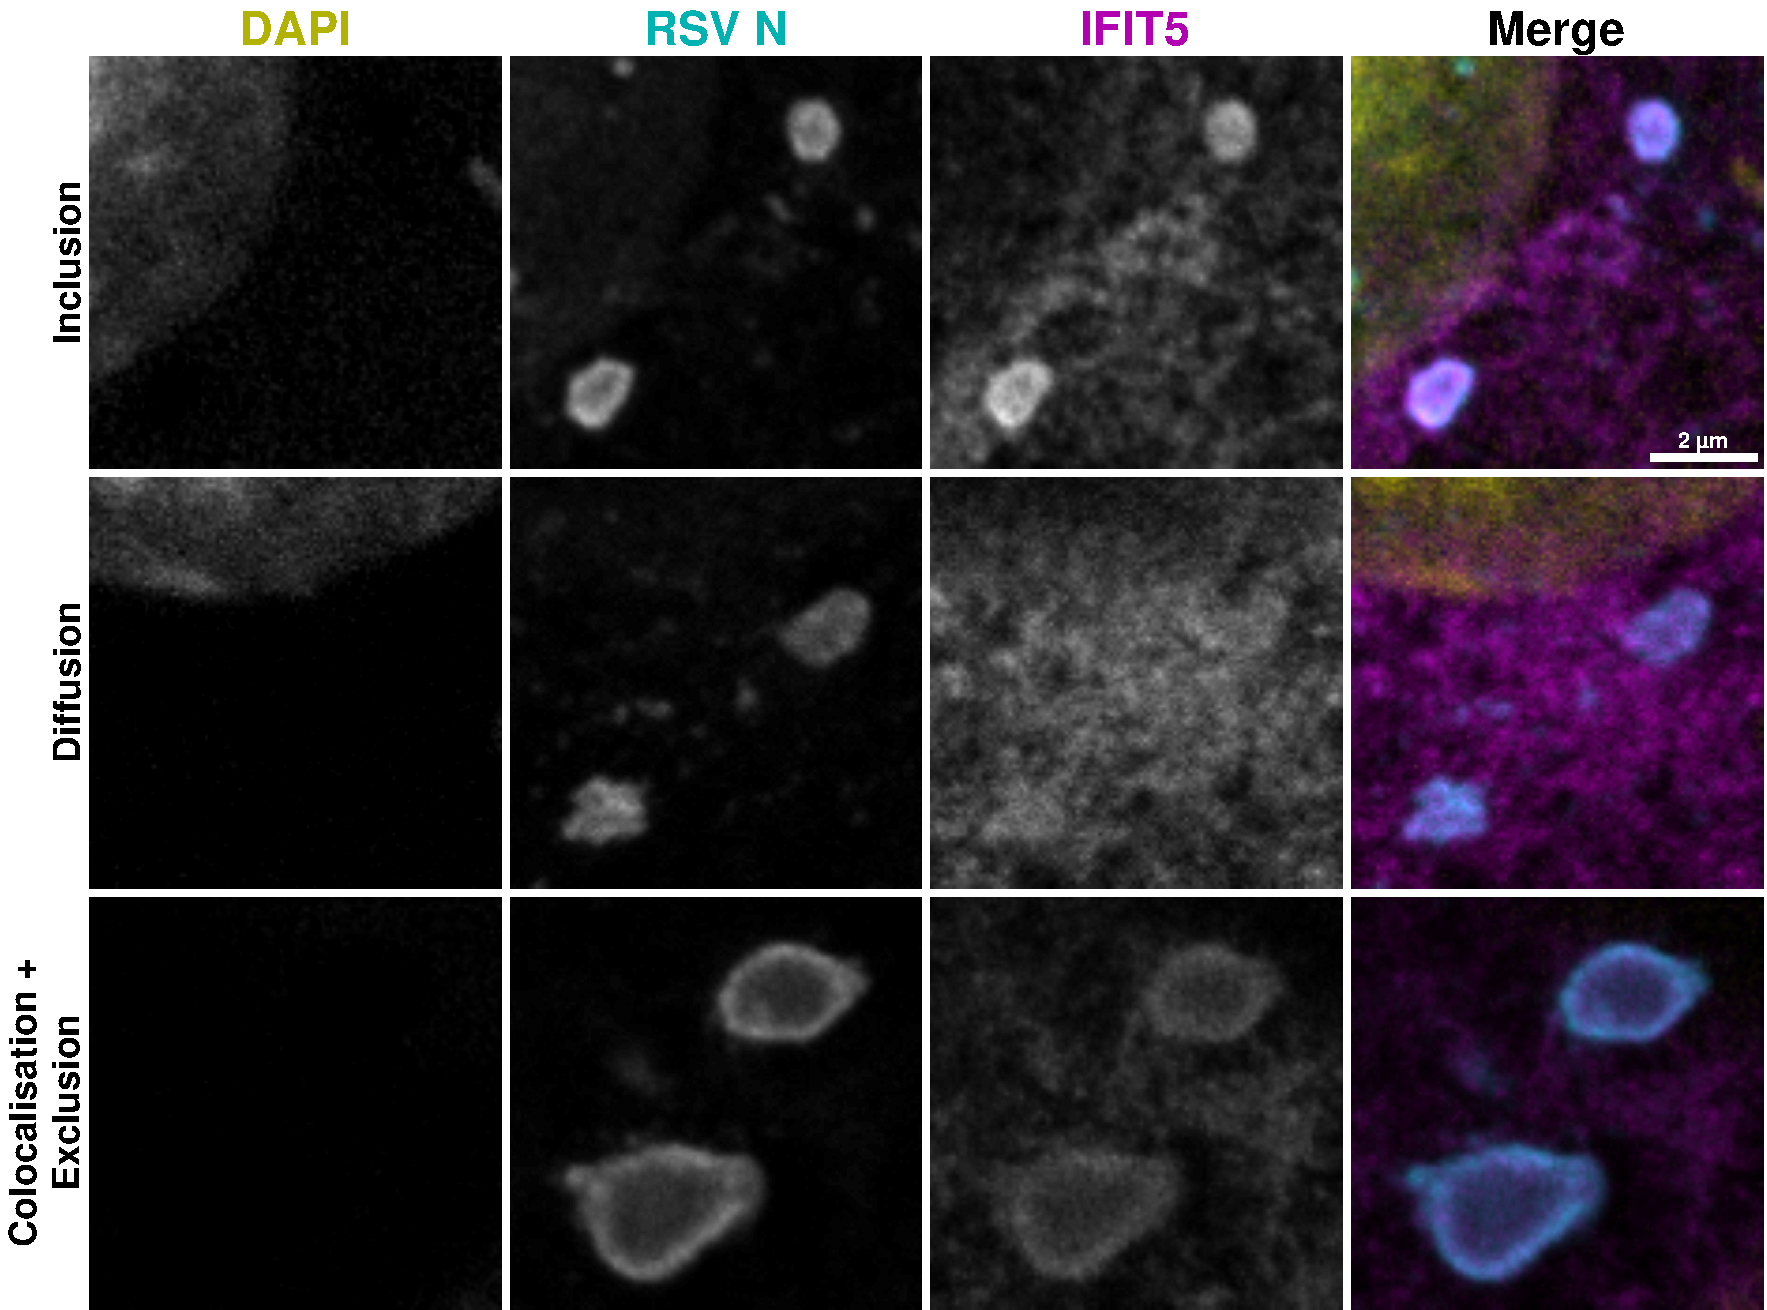
\includegraphics[width=1\linewidth]{08. Chapter 3/Figs/04. Overexpression/04. IFIT5/03. i5-hrsv.pdf}
    \caption[Representative Images of Observed Phenotypes of Exogenous hIFIT5 in the Context of hRSV Inclusion Bodies in VERO Cell Line.]{\textbf{Representative Images of Observed Phenotypes of Exogenous hIFIT5 in the Context of hRSV Inclusion Bodies in VERO Cell Line.} Vero cells were infected with human RSV at MOI 1. 24 HPI, the cells were transfected with hIFIT5-FLAG containing plasmids using TransIT-X2 and were fixed after further 24 hours. Cellular nuclei were stained with DAPI (yellow), and cells were double-labeled with anti-RSV N (cyan) and anti-FLAG (magenta) antibodies. This figure showcases representative examples of relevant phenotypes in the interaction between exogenous hIFIT5 and hRSV inclusion bodies. These phenotypes are presented in descending order based on their percentage proportions. The scale bar indicates 2 \(\mu m\).}
    \label{fig:Representative Images of Observed Phenotypes of Exogenous hIFIT5 in the Context of hRSV Inclusion Bodies in VERO Cell Line}
\end{figure}

45 26 26

0.7 1.2 6

\begin{figure}
    \begin{subfigure}{0.495\textwidth}
        \caption{}
        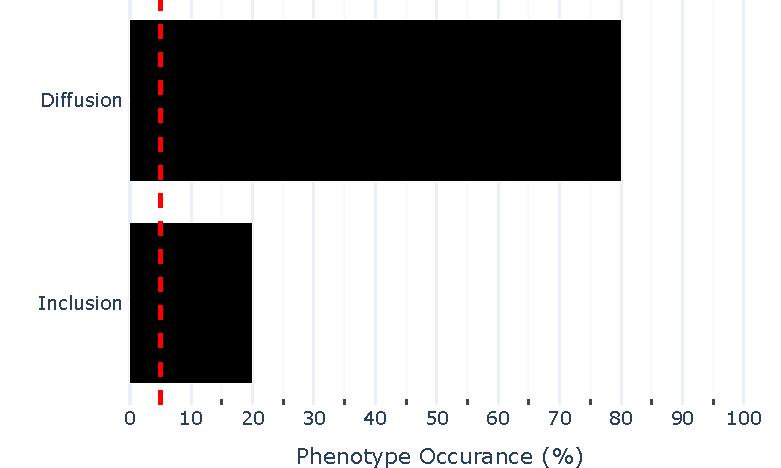
\includegraphics[width=1\linewidth]{08. Chapter 3/Figs/04. Overexpression/04. IFIT5/04. bar_i5_brsv.pdf} 
    \end{subfigure}
    \begin{subfigure}{0.495\textwidth}
        \caption{}
        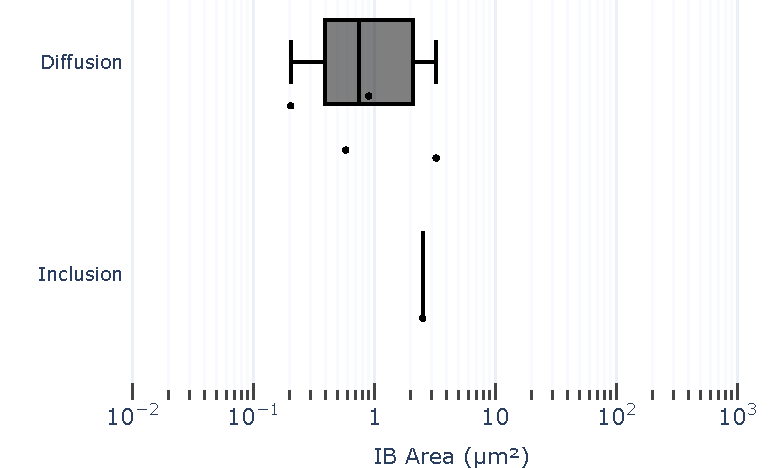
\includegraphics[width=1\linewidth]{08. Chapter 3/Figs/04. Overexpression/04. IFIT5/05. box_i5_brsv.pdf}
    \end{subfigure}
    \caption[Observed Phenotypes of Exogenous hIFIT5 in the Context of bRSV Inclusion Bodies in VERO Cell Line.]{\textbf{Observed Phenotypes of Exogenous hIFIT5 in the Context of bRSV Inclusion Bodies in VERO Cell Line.} Vero cells were infected with bovine RSV at MOI 1. 24 HPI, the cells were transfected with hIFIT5-FLAG containing plasmids using TransIT-X2 and were fixed after further 24 hours. Cells were labeled with anti-RSV N and anti-FLAG antibodies and imaged on confocal microscope. Panel (a) shows percentual proportions of observed phenotypes between bRSV inclusion bodies and exogenous hIFIT5 (5 observations), with the red dotted line denoting the 5\% threshold, marking phenotypes considered relevant above this limit. Panel (b) shows the IB area in \(\mu m^2\) per observed relevant phenotype.}
    \label{fig:Observed Phenotypes of Exogenous hIFIT5 in the Context of bRSV Inclusion Bodies in VERO Cell Line}
\end{figure}

\begin{figure}
    \centering
    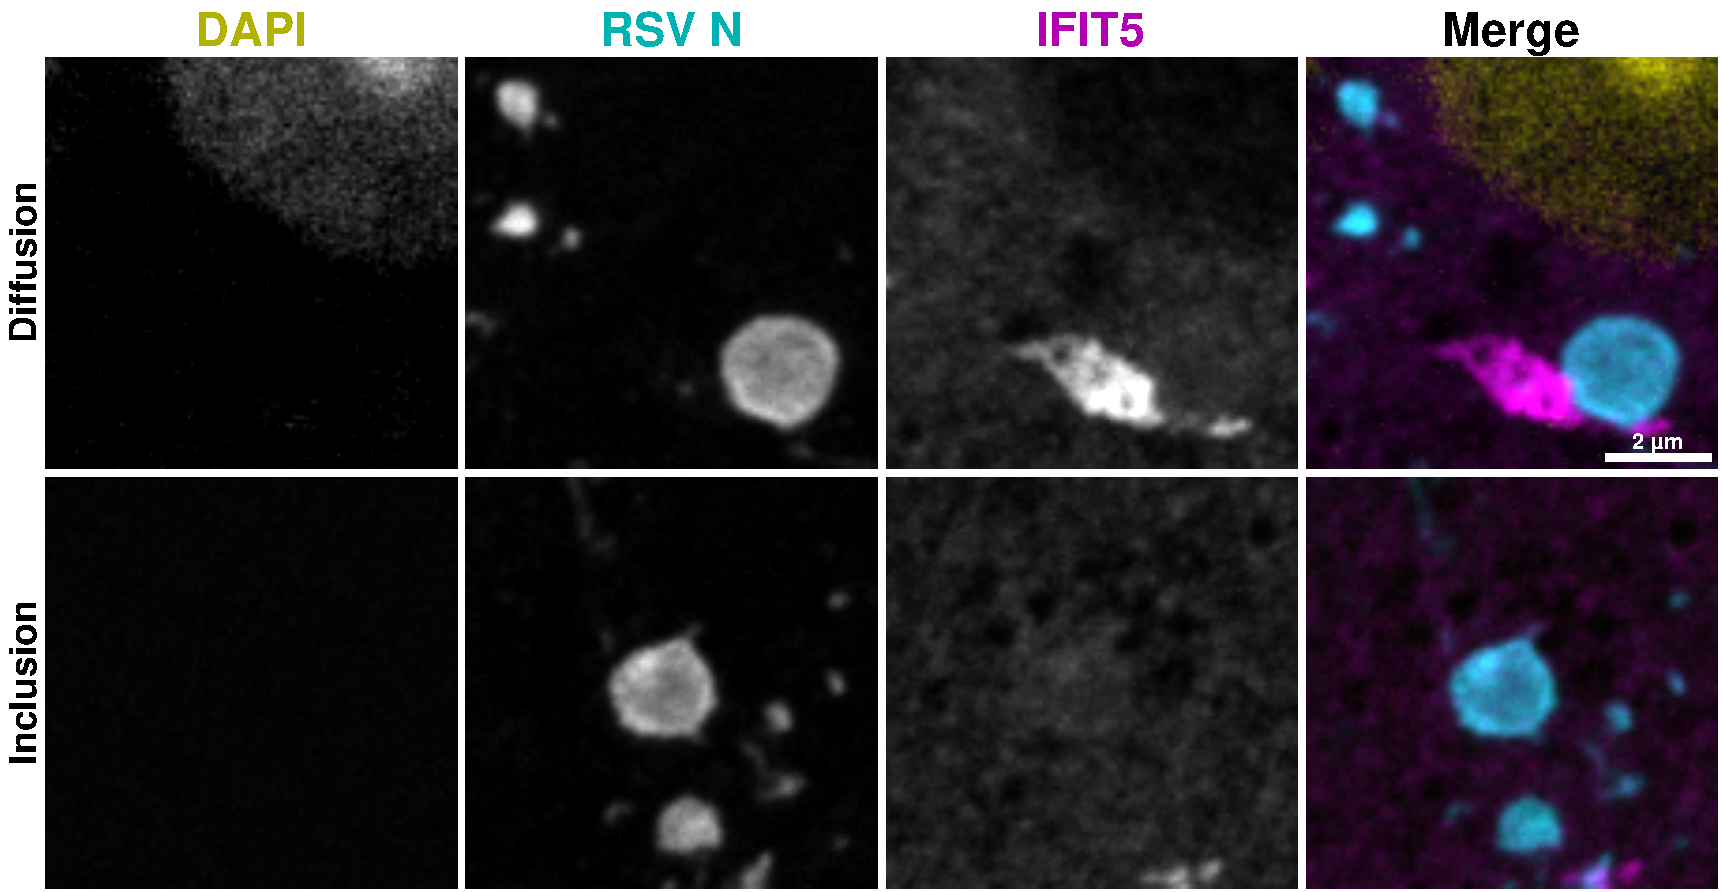
\includegraphics[width=1\linewidth]{08. Chapter 3/Figs/04.  Overexpression/04. IFIT5/06. i5-brsv.pdf}
    \caption[Representative Images of Observed Phenotypes of Exogenous hIFIT5 in the Context of bRSV Inclusion Bodies in VERO Cell Line.]{\textbf{Representative Images of Observed Phenotypes of Exogenous hIFIT5 in the Context of bRSV Inclusion Bodies in VERO Cell Line.} Vero cells were infected with bovine RSV at MOI 1. 24 HPI, the cells were transfected with hIFIT5-FLAG containing plasmids using TransIT-X2 and were fixed after further 24 hours. Cellular nuclei were stained with DAPI (yellow), and cells were double-labeled with anti-RSV N (cyan) and anti-FLAG (magenta) antibodies. This figure showcases representative examples of relevant phenotypes in the interaction between exogenous hIFIT5 and bRSV inclusion bodies. These phenotypes are presented in descending order based on their percentage proportions. The scale bar indicates 2 \(\mu m\).}
    \label{fig:Representative Images of Observed Phenotypes of Exogenous hIFIT5 in the Context of bRSV Inclusion Bodies in VERO Cell Line}
\end{figure}

80 20

0.7 2.5

\begin{figure}
    \begin{subfigure}{0.495\textwidth}
        \caption{}
        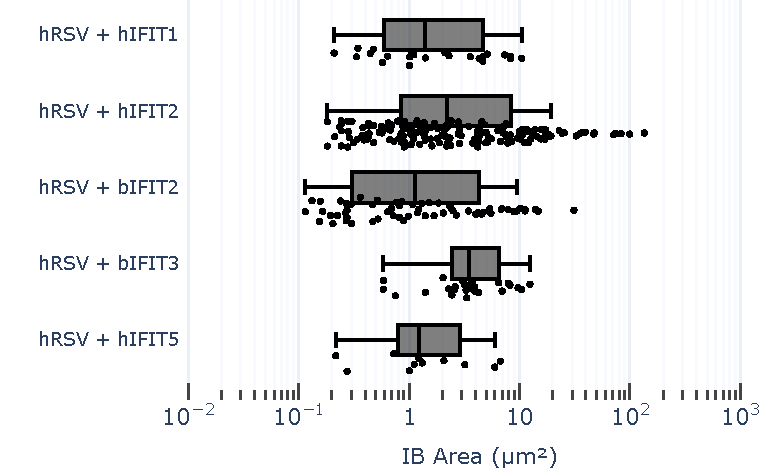
\includegraphics[width=1\linewidth]{08. Chapter 3/Figs/04. Overexpression/01. sizes-oe-hrsv.pdf} 
    \end{subfigure}
    \begin{subfigure}{0.495\textwidth}
        \caption{}
        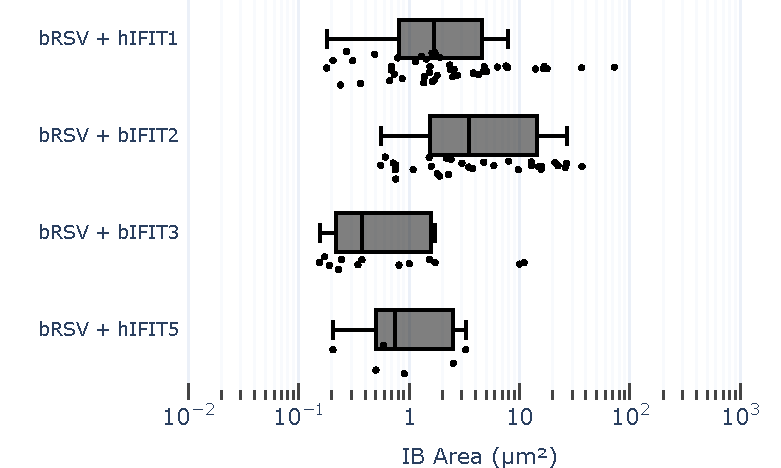
\includegraphics[width=1\linewidth]{08. Chapter 3/Figs/04. Overexpression/02. sizes-oe-brsv.pdf}
    \end{subfigure}
    \caption[sizes between ifits.]{\textbf{sizes between ifits.} comparasion of sizes of IBs}
    \label{fig:sizes between ifits}
\end{figure}


% summary
Overexpressed hIFIT1-FLAG in the context of h/bRSV infection colocalises to both human and bovine IB structures.

Overexpressed bIFIT3 behaves equally between hRSV and bRSV infection, that is it sometimes colocalises with the IB structure and sometimes is completely excluded from the structure.

Overexpressed hIFIT5 in hRSV infected cells colocalises with the IBs.
